\documentclass[11pt,letterpaper]{article}
\usepackage[margin=1in]{geometry}
\usepackage[T1]{fontenc}
\usepackage{lmodern}
\usepackage{amsmath,amssymb,amsthm,booktabs,graphicx}
\usepackage[round,authoryear]{natbib}
\usepackage[colorlinks=true,allcolors=blue]{hyperref}
\usepackage{microtype}
\hypersetup{pdftitle={Total Error: What Classifier Validation Establishes About Exposure Comparisons},
  pdfauthor={Gaurav Sood}}
\newcommand{\OriginalObservationCorrelation}{0.900}
\newcommand{\OriginalMeanCorrelation}{0.901}
\newcommand{\OriginalTotalCorrelation}{0.538}
\newcommand{\OriginalMeanError}{51.239}
\newcommand{\ConstantTotalCorrelation}{0.537}
\newcommand{\TheoreticalTotalCorrelation}{0.553}

\newcommand{\BenchmarkUsers}{1,132}
\newcommand{\BenchmarkDomains}{34,078}
\newcommand{\BenchmarkRecords}{103,853}
\newcommand{\BenchmarkVisits}{4,767,099}
\newcommand{\BenchmarkContrasts}{84}
\newcommand{\FocalTruth}{0.828}
\newcommand{\FocalLower}{-17.00}
\newcommand{\FocalUpper}{16.72}
\newcommand{\FocalAdverseLower}{-21.05}
\newcommand{\FocalAdverseUpper}{20.16}
\newcommand{\SmallAuditCoverage}{93.1}
\newcommand{\SmallAuditCoverageLower}{91.3}
\newcommand{\SmallAuditCoverageUpper}{94.6}
\newcommand{\LargeAuditCoverage}{95.6}
\newcommand{\LargeAuditWidth}{1.40}
\newcommand{\RareNormalCoverage}{91.97}

\newtheorem{proposition}{Proposition}
\newcommand{\E}{\operatorname{E}}
\newcommand{\Var}{\operatorname{Var}}
\newcommand{\Cov}{\operatorname{Cov}}
\newcommand{\Corr}{\operatorname{Corr}}
\title{Total Error: What Classifier Validation Establishes About Exposure Comparisons}
\author{Gaurav Sood\thanks{\href{mailto:gsood07@gmail.com}{gsood07@gmail.com}.
The argument about browsing volume and costly errors on popular domains appears
in the June 2020 manuscript coauthored with Suriyan Laohaprapanon
\citep{laohaprapanon2020domain}. The standalone note and original simulation
were added in June 2023. This revision corrects the error-rate definitions
and develops the validation bounds and inference results. Code and history:
\url{https://github.com/finite-sample/total_error}.}}
\date{}
\begin{document}
\maketitle

\begin{abstract}
A classifier's confusion matrix need not validate comparisons constructed from
its predictions. When domain labels are reused across browsing histories, the
estimand determines a signed, weighted sum of domain mistakes. Its bias and
variance depend on the full joint error distribution across domains. I characterize the
sharp bounds on this error given exact target-population confusion counts and
show when those counts identify a comparison. The decisive restriction is
constant influence within each partially erroneous stratum. A finite-population
audit gives simultaneous bounds for linear comparisons, but projecting count
information can discard enough information that interval width remains positive
even as the audit grows. Direct estimation of weighted errors avoids that loss.
A reproducible browsing-data stress test illustrates the distinction, while
an exact rare-error example shows why many contributing domains alone do not
justify normal inference. The results clarify what validation must retain when
predictions become research outcomes.
\end{abstract}

A researcher labels websites and combines those labels with browsing records
to compare exposure across demographic groups. An accurate classifier seems
to provide reassurance. Yet accuracy counts domains equally, whereas each
comparison attaches its own signed weights to the same labels. A mistake on
a domain visited disproportionately by one group can matter more than many
correct labels elsewhere. Because users share labels and different domains can share classifier
failures, measurement errors can be dependent even between users who visit
different sites. Both bias and uncertainty depend on where errors occur.

This note asks what even an exactly known target-population confusion matrix
establishes about such comparisons. The answer is a sharp identification
interval obtained by sorting the comparison's domain weights. The interval
collapses precisely when weights are constant within every prediction stratum
with an interior error count. This characterization separates a shortage of
validation observations from information lost by summarizing those observations
as counts. It also explains why a count-based audit can remain imprecise after
the aggregate error fraction is accurately learned.

The problem intersects several established literatures. Quantification estimates
population label prevalence from predictions and error rates
\citep{vaz2019quantification}; prevalence uses equal domain weights, whereas
exposure comparisons use heterogeneous, often signed weights. Shared domain
errors have the same linear propagation structure that motivates attention to
common shocks in shift-share inference \citep{adao2019}. Multiaccuracy already
expresses validation through residual moments for relevant functions
\citep{kim2019}. Design-based supervised learning supplies unbiased corrections
from probability samples of verified labels \citep{egami2023}, and election and
financial auditing already address bounded weighted errors using random audits
\citep{stark2008audits,shekhar2023audits}. Neither covariance propagation nor the
difference estimator is a new result here. The contribution is the explicit
characterization of what confusion summaries retain for reused labels, its
limits for auditing, and a reproducible assessment on exposure comparisons.

\section{Start with the estimand}\label{sec:estimand}
Suppose the research question concerns a difference in exposure between two
groups, or a demographic coefficient in a regression of exposure. Define that
quantity before assessing the classifier. Let $C=(c_{ij})$ contain visits by
$n$ users to $k$ domains, and let $y_j\in\{0,1\}$ be domain $j$'s true label.
The true exposure vector is $T=Cy$. For declared user weights $a$, the estimand is
\begin{equation}\label{eq:estimand}
 \theta=a^{\mathsf T}T=a^{\mathsf T}Cy=w^{\mathsf T}y,
 \qquad w=C^{\mathsf T}a.
\end{equation}
For a difference of group means, $a_i=1/n_A$ in group $A$ and $a_i=-1/n_B$
in group $B$. A single user's total sets that user's weight to one and all
others to zero. For exposure shares, first replace $C$ by
$\operatorname{diag}(V_1^{-1},\ldots,V_n^{-1})C$, where $V_i=\sum_jc_{ij}>0$;
the same mapping then gives the domain weights for the chosen share comparison.
Replacing visits by duration changes the exposure unit but not the mapping.

Regression coefficients are also fixed linear functionals of the labels.
For a full-rank demographic design $X$, write
$A=(X^{\mathsf T}X)^{-1}X^{\mathsf T}$ and define the complete-label coefficient
$\beta^*=ACy$. A coefficient contrast $r^{\mathsf T}\beta^*$ has user weights
$a=A^{\mathsf T}r$ and domain weights $w=C^{\mathsf T}A^{\mathsf T}r$.
These are descriptive coefficients for the specified browsing frame; causal or
population interpretations require additional assumptions. Throughout, the
browsing matrix, comparison weights, and regressors are fixed. Their uncertainty,
if relevant to the research question, requires an additional sampling model.
Domain labels also define the construct: they measure visits to domains with a
given label, not necessarily consumption of that content on mixed-content sites.

Let $q\in\{0,1\}^k$ contain predicted labels, $q_j=\widehat y_j$, and let
$e=q-y$. The predicted exposure vector is $\widehat T=Cq$. The predicted
comparison is $\widehat\theta=w^{\mathsf T}q$, so its error is exactly
\begin{equation}\label{eq:contrast}
 \Delta=\widehat\theta-\theta=w^{\mathsf T}e.
\end{equation}
Thus it is the estimand that determines which classification mistakes matter.
A popular domain can dominate an individual's total but cancel from a group
comparison if the groups use it equally. Conversely, a less popular domain
visited disproportionately by one group can be influential for that comparison.
An error rate that weights all domains equally need not describe either target.

For a fixed fitted classifier and fixed labels, $\Delta$ is fixed. To discuss
bias and variance, specify a repeated-prediction process, such as repeated
training samples, while fixing $C,y,a$ and, where used, $X,r$. All moments below
condition on this fixed design. Define $b=\E[e]$ and the full joint covariance
$\Sigma=\Cov(e)$, without assuming independence across domains. Then
\begin{align}
 \operatorname{Bias}(\widehat\theta)&=w^{\mathsf T}b,\notag\\
 \Var(\Delta)&=w^{\mathsf T}\Sigma w
 =\sum_jw_j^2\Sigma_{jj}
   +2\sum_{j<\ell}w_jw_\ell\Sigma_{j\ell},\label{eq:targetmoments}\\
 \E[\Delta^2]&=(w^{\mathsf T}b)^2+w^{\mathsf T}\Sigma w.
 \label{eq:targetrisk}
\end{align}
Equations~\eqref{eq:estimand}--\eqref{eq:targetrisk} connect the research quantity
to its domain weights, its systematic error, and its uncertainty. Covariance
between domain errors is part of the estimand's error from the outset.
Dependence alone does not determine bias; systematically misclassifying domain
types used disproportionately by one group can make $w^{\mathsf T}b$ nonzero.

User totals and regression vectors are corresponding joint quantities. Writing
$d=\widehat T-T$ and $\widehat\beta=ACq$ gives
\begin{align}
 d&=Ce,\label{eq:identity}\\
 \E[d]&=Cb, & \Cov(d)&=C\Sigma C^{\mathsf T},\label{eq:moments}\\
 \E[\widehat\beta-\beta^*]&=ACb,
 &\Cov(\widehat\beta-\beta^*)&=AC\Sigma C^{\mathsf T}A^{\mathsf T}.
 \label{eq:regression}
\end{align}
The same domain error is reused across all visits and users. These formulas
quantify the specified prediction-error process; they do not include browsing-log
error, user sampling, or uncertainty about the construct. They concern predicted
exposure as an outcome. Noisy exposure as a regressor is a different
errors-in-variables problem \citep{fong2021predictions}.

\section{Dependence follows the domain weights}\label{sec:dependence}
There are two sources of dependence. A domain's label is reused across users,
and different domains are classified by the same fitted model. Shared training
data, model parameters, and similar content or site templates can cause errors
to move together under repeated fitting. Distinct domain names do not establish
independent errors. Users need not visit the same domains to have correlated
measurement errors: visiting different domains whose errors covary is enough.
In equation~\eqref{eq:targetmoments}, positively correlated mistakes increase
variance when their domain weights have the same sign, and decrease it when
the weights have opposite signs.

For a limiting example, suppose centered errors are shared within domain
families: $e_j-b_j=u_{g(j)}$, with independent family shocks $u_g$ of variance
$\tau_g^2$. This is compatible with binary predictions when the classifier
assigns one common random prediction to every domain in a family. Then
\begin{equation}\label{eq:families}
 \Var(\Delta)=\sum_g\tau_g^2
                 \left(\sum_{j:g(j)=g}w_j\right)^2.
\end{equation}
A family of $m$ domains with unit weights contributes $m^2\tau_g^2$, whereas
assuming independent domain errors would give $m\tau_g^2$. Signed weights can
instead cancel within a family. The relevant concentration is in aggregate
family influence, not just individual domain influence. This example is a
special covariance structure, not an assertion that the right families are
known or that all within-family mistakes are perfectly correlated.

Independent domain errors are another special case: $\Sigma$ is diagonal,
with entries $v_j$. For user totals, equation~\eqref{eq:moments} reduces to
\begin{equation}\label{eq:covariance}
 \Var(d_i)=\sum_jc_{ij}^2v_j,\qquad
 \Cov(d_i,d_\ell)=\sum_jc_{ij}c_{\ell j}v_j.
\end{equation}
Let $\alpha_j$ be the false-positive probability on a truly negative domain
and $\beta_j$ the false-negative probability on a truly positive domain.
For binary predictions, $v_j=\alpha_j(1-\alpha_j)$ on negative domains and
$v_j=\beta_j(1-\beta_j)$ on positive domains. Repeated visits multiply one
classification error; treating visits as independent would incorrectly replace
squared visit weights by visit counts. Even this special case induces dependence
across users who share uncertain domains.

An uncertainty procedure must follow the same structure as the estimand.
Resampling users while holding predictions fixed does not propagate repeated-
training uncertainty. Each replicate must preserve shared labels across users
and the joint distribution of errors across domains. Independently perturbing
each domain label imposes a diagonal $\Sigma$; resampling the classifier fit
and predicting all domains together can preserve dependence induced by that
fitting process, provided the resampling scheme represents that process.
A prediction-error covariance cannot simply be added to an arbitrary reported
regression covariance: the components may overlap or be dependent. Neither
larger user samples nor user-level clustering alone guarantees that this error
disappears,
and standard errors do not repair bias.

\subsection{Many domains do not ensure a normal approximation}
Even with independent domain errors, diffuse variance shares alone do not
justify Gaussian inference. Let all true labels be zero and let each of $k$
domains be falsely labeled positive independently with probability $1/k$.
With $w_j=1$, total error $B_k$ is binomial with mean one and variance $1-1/k$.
The largest domain variance share is $1/k$, yet
$B_k-1\Rightarrow\operatorname{Poisson}(1)-1$, not a normal distribution.
At $k=10{,}000$, an oracle interval using the exact bias and variance but a
normal 1.96 cutoff has coverage \RareNormalCoverage{}\%. This calculation
uses exact binomial probabilities, not simulation.

For independent bounded binary errors, a sufficient Lindeberg condition is
\[\frac{\max_j|w_j|}{\sqrt{\sum_jw_j^2v_j}}\to0.\]
A small maximum variance share
$\max_j w_j^2v_j/\sum_jw_j^2v_j$ is weaker when errors become rare. The example
violates the former condition and satisfies the latter. A growing number of
domains cannot substitute for a condition on the distribution of their errors.
This is a prediction-error example, distinct from the fixed-label audit design.

\section{What a confusion matrix identifies}\label{sec:identification}
A confusion matrix can be exactly correct for the target domains and still fail
to determine a user comparison. This is an information problem before it is a
sampling problem. Fix the predictions $q$ and the domain weights $w$ induced
by the estimand in equation~\eqref{eq:estimand}. We now ask what a validation
summary establishes about the fixed target $\theta=w^{\mathsf T}y$, without
specifying a stochastic model for how the classifier's mistakes were generated.

Let $P=\{j:q_j=1\}$ and $N=\{j:q_j=0\}$. Suppose the entire target-population
confusion matrix is known: $f$ predictions in $P$ are false positives and $g$
predictions in $N$ are false negatives. This grants more information than ordinary
held-out validation, whose error rates require a transport assumption.
For a finite collection $B$ of weights, let $S_-(B,m)$ and $S_+(B,m)$ denote
the sums of its $m$ smallest and largest elements, with a zero sum when $m=0$.

\begin{proposition}[Sharp bounds from confusion counts]\label{prop:bounds}
Across binary label vectors compatible with $q,f,g$, the smallest and largest
possible errors $\Delta=\widehat\theta-\theta$ are
\begin{align}
 L&=S_-(w_P,f)-S_+(w_N,g),\notag\\
 U&=S_+(w_P,f)-S_-(w_N,g).
\end{align}
Consequently $[\widehat\theta-U,\widehat\theta-L]$ is the smallest interval
containing every compatible value of $\theta$. Both endpoints are attainable.
\end{proposition}
\begin{proof}
Only false positives and false negatives contribute:
$\Delta=\sum_{j\in\mathrm{FP}}w_j-\sum_{j\in\mathrm{FN}}w_j$.
Select $f$ indices from $P$ and $g$ from $N$. The two selections have disjoint
supports and no other restrictions. Selecting the smallest positive-stratum
weights and largest negative-stratum weights minimizes the error; reversing
these selections maximizes it. Assign the selected indices the corresponding
true labels to attain each endpoint.
\end{proof}
The compatible values form a finite set, so the interval is its convex hull;
not every interior value need be attainable. A reported sign is established by
these counts only if the bounding interval excludes zero. The calculation
requires sorting, rather than a general integer-programming solver.

For example, take $q=(1,1,0,0)$, $w=(1,-1,1,-1)$, and $f=g=1$.
The same confusion matrix permits errors of $-2$, $0$, and $2$.
Prevalence, accuracy, FPR, and FNR are identical across those assignments.
Adding correctly classified domains with zero contrast weight makes accuracy
arbitrarily close to one without resolving the comparison. These are domains
that can affect individual exposure but cancel from the chosen contrast.

\begin{proposition}[When counts suffice]\label{prop:sufficient}
In a stratum of $M$ domains sharing the same predicted label, with exactly
$m$ errors, the error sum is
point identified if and only if $m\in\{0,M\}$ or all its contrast weights are
equal. Its identification width obeys
\begin{equation}\label{eq:dispersion}
 S_+(w,m)-S_-(w,m)
 \leq \min(m,M-m)\{\max_jw_j-\min_jw_j\}.
\end{equation}
Widths add across strata. For several comparisons, counts determine every
comparison if and only if their vector of domain weights is constant within
each stratum with an interior error count.
\end{proposition}
\begin{proof}
Constant weights, no errors, and all errors each determine the sum. If
$0<m<M$ and two weights differ, choose an error set containing one of those
indices but not the other. Exchanging them changes the sum, proving necessity.
The difference between two sums of $m$ terms is at most $m$ times the range.
Taking complements gives the corresponding bound with $M-m$ terms. The
vector statement applies the exchange argument to each coordinate.
\end{proof}
For a stratum mixing predicted labels, the corresponding criterion applies to
the signed contributions $(2q_j-1)w_j$, not to $w_j$ alone.
The result specifies what a finer validation table must preserve. Stratifying
by predicted label alone is sufficient only when the contrast attaches equal
weights within each partially erroneous stratum. Partitioning domains by
similar contrast weights can reduce ambiguity; bins chosen for one comparison
need not work for another. Error rates conditional on user demographics are
not automatically available, because the same domain can enter many groups.

\section{Auditing the target domains}\label{sec:audit}
A target-domain audit can convert these bounds into confidence intervals.
The construction below uses established finite-population counting and audit
ideas. Sorting worst-case error contributions and checking them by random
audits has close precedents in election auditing \citep{stark2008audits}.
Weighted finite-population inference with prediction side information is also
an established problem \citep{shekhar2023audits}. The purpose here is to expose
what confusion-count evidence preserves about reusable predictions, not to
claim a new general audit principle or an optimal interval.

Partition the domains into strata $h=1,\ldots,H$ using information known before
labels are audited. Draw a simple random sample without replacement of a fixed
size $n_h$ from the $M_h$ domains in each stratum. Let $K_h$ be its unknown
number of incorrect predictions and $X_h$ the observed audit-error count.
Conditional on the fixed labels and predictions,
\begin{equation}
 X_h\sim\operatorname{Hypergeometric}(M_h,K_h,n_h).
\end{equation}
Choose nonnegative error budgets $\delta_h$ summing to at most $\delta$.
Retain each feasible integer $K$ for which both
$\Pr_K(X_h\leq x_h)\geq\delta_h/2$ and
$\Pr_K(X_h\geq x_h)\geq\delta_h/2$.
Write the smallest and largest retained integers as $\ell_h,u_h$.
A census stratum reveals $K_h=x_h$ exactly and needs no error budget; an
unaudited stratum contributes no count restriction.

Let $O$ be the audited domains and $U_h$ the unaudited domains in stratum $h$.
Set $c_j=(2q_j-1)w_j$ and
$d_O=\sum_{j\in O}w_j(q_j-y_j)$. Define
\begin{align}
 L_A&=d_O+\sum_h\min_{\ell_h-x_h\leq m\leq u_h-x_h}
                 S_-(c_{U_h},m),\notag\\
 U_A&=d_O+\sum_h\max_{\ell_h-x_h\leq m\leq u_h-x_h}
                 S_+(c_{U_h},m),\label{eq:auditbounds}
\end{align}
where the optimization is over integers. Signed weights make this optimization
necessary: an extreme need not occur at the largest admissible error count.

\begin{proposition}[A simultaneous audit certificate]\label{prop:audit}
Under the fixed stratified sampling design, the interval
$[\widehat\theta-U_A,\widehat\theta-L_A]$ covers the fixed true contrast with
probability at least $1-\delta$. The same event guarantees coverage for every
linear contrast of this one label vector. The endpoints are sharp over the
binary configurations satisfying the count intervals and all audited labels.
\end{proposition}
\begin{proof}
Inverting each pair of hypergeometric tails excludes the true $K_h$ with
probability at most $\delta_h$. A union bound therefore includes all true
counts with probability at least $1-\delta$. On that event, the true errors in
$U_h$ number between $\ell_h-x_h$ and $u_h-x_h$. Sorting and choosing a count
in that range gives the extrema in equation~\eqref{eq:auditbounds}; the choices
are independent restrictions across strata and hence jointly attainable.
The true label vector lies in the same configuration set for every choice of
$w$, which establishes simultaneous coverage.
\end{proof}
The labels and predictions are fixed under this design: systematic or correlated
classifier mistakes do not invalidate the guarantee. Coverage is over repeated
audit samples, not conditional on the realized
sampled identities. It requires neither independent classification errors nor
a large-domain Gaussian approximation. The count confidence region can be
conservative, and sharp projection of that region does not make the resulting
confidence interval shortest. The guarantee concerns one outcome; combining
separate audits of several outcomes requires an additional simultaneous-error
allocation. Optional stopping, adaptive strata, and imperfect audit labels
require further assumptions or other audit procedures.

\paragraph{The information discarded by count projection.}
A large audit need not make these intervals narrow. To see this, let all $N$
predictions equal one, half the weights equal $1/N$ and half equal $-1/N$.
Suppose a fraction $p<1/2$ of labels in each half are wrong. The true contrast
is zero. If $n\to\infty$ but $n/N\to0$, an unstratified audit consistently
learns the overall error fraction. Yet unaudited errors can still be placed
almost entirely on either weight sign: the projected interval width converges
to $2p$. A direct estimate of the weighted audit residual instead has standard
error of order $n^{-1/2}$. Separating the two weight signs into strata removes
this particular information loss. The distinction is between estimating a
weighted residual and bounding it after retaining only counts.

For a declared contrast, an ordinary stratified difference estimator uses
$z_j=w_j(y_j-q_j)$ directly:
\begin{equation}\label{eq:stratified}
 \widetilde\theta=\widehat\theta+
 \sum_h\frac{M_h}{n_h}\sum_{j\in O_h}z_j,\qquad
 \widehat V=\sum_h\frac{M_h^2(1-n_h/M_h)}{n_h}s_{z,h}^2,
\end{equation}
where $s_{z,h}^2$ is the sample variance and a census stratum contributes zero
variance. Under independent stratum draws, the estimate and variance estimator
are design unbiased, with at least two audited domains in each noncensus
stratum. Normal intervals need a separate approximation. A conservative
finite-sample alternative applies Hoeffding's without-replacement inequality
\citep{hoeffding1963} to each bounded residual mean and sums the stratum radii.
More efficient weighted audit procedures are available \citep{shekhar2023audits}.
The count certificate is useful for interpreting validation summaries and
covering many comparisons together, not a general replacement for direct
inference about a chosen comparison.


\section{A browsing-data stress test}\label{sec:benchmark}
The empirical question is how much information confusion counts retain for
comparisons supported by an actual browsing matrix. The fixed benchmark contains
\BenchmarkUsers{} pseudonymized users, \BenchmarkDomains{} domains,
\BenchmarkRecords{} user--domain records, and \BenchmarkVisits{} visits.
It is the bundled \texttt{fewlab} extract of the June 2022 YouGov Pulse/RealityMine
panel with Blacklight scanner outcomes. The replication package pins the source
commit and file hashes. Its analytic universe contains domains with recorded
scanner labels; exposure shares use visits within that universe as their
denominator. These recorded outcomes are reference labels for the experiment,
not error-free measures of all tracking activity. The exercise makes no causal
or population-representative claim about demographic differences.

We retain the extract's demographic design matrix: an intercept and indicators
for gender, race, education, and source-coded age groups. Omitted categories are Male, White,
HS or Below, and under 25. For each of seven scanner outcomes, we
calculate all twelve non-intercept least-squares coefficients for both visit
totals and visit shares. Each coefficient is a fixed weighted label sum.
Two scanner columns are counts and are dichotomized at a positive value; the
other five are binary. Complete labels, valid joins, positive visits, and full
column rank are checked before estimation.

Predictions are imposed, rather than produced by a fitted classifier. Within
each true class, we randomly flip the integer part of 1\%, 5\%, or 10\% of the
labels. We then perform two distinct exercises. First, holding those predictions
fixed, Proposition~\ref{prop:bounds} gives the true-coefficient range compatible
with their exact confusion counts. Second, holding the reference labels fixed,
we rearrange the same numbers of false positives and false negatives to minimize
or maximize the predicted coefficient. The latter asks whether two classifiers
with identical confusion matrices can report opposing comparisons. It is a
worst-case sensitivity analysis, not an estimate of likely classifier bias.
Extrema are computed separately for each coefficient; a single error arrangement
need not reverse all comparisons at once.

\begin{table}[htbp]
\centering\small
\caption{What exact confusion counts establish at 1\% imposed error in each true class}
\label{tab:browsing}
\begin{tabular}{lrrr}
\toprule
Scanner outcome & Sign identified & Reversal possible & Median width (pp) \\
\midrule
Advertising trackers & 0/12 & 12/12 & 47.8 \\
Third-party cookies & 0/12 & 12/12 & 52.5 \\
Canvas fingerprinting & 0/12 & 12/12 & 29.5 \\
Session recording & 0/12 & 12/12 & 31.6 \\
Key logging & 0/12 & 12/12 & 21.3 \\
Facebook pixel & 0/12 & 12/12 & 43.6 \\
Google Analytics & 0/12 & 12/12 & 21.6 \\
\bottomrule
\end{tabular}

\par\smallskip
\begin{minipage}{\linewidth}\footnotesize
Each row covers twelve demographic coefficients of visit shares in the fixed
browsing frame. ``Sign identified'' counts bounding intervals excluding zero
for fixed random predictions. ``Reversal possible'' counts coefficients for
which rearranging errors with the same confusion matrix can reverse the
reference coefficient's sign. Median width summarizes identification intervals,
measured in percentage points (pp); these are not sampling intervals. Error
counts are rounded down within each true class. All outcomes, coefficients,
scales, and error fractions are included in the machine-readable results.
\end{minipage}
\end{table}

At the smallest imposed error fraction, none of the \BenchmarkContrasts{}
share-coefficient signs is identified by the full confusion matrix
(Table~\ref{tab:browsing}); all permit a sign reversal by rearranging errors.
The corresponding total coefficients show the same pattern, as do the larger
error fractions. This establishes a limitation of confusion summaries for
this frame. It does not establish that actual classifiers make such adverse
errors. For example, the reference female coefficient for Facebook-pixel visit
share is \FocalTruth{} percentage points. For the fixed random predictions,
its count-compatible interval is $[\FocalLower{},\FocalUpper{}]$ percentage
points. Holding the reference labels fixed instead, moving the same errors
can produce predicted coefficients from \FocalAdverseLower{} to
\FocalAdverseUpper{} percentage points.

\subsection{What an audit recovers}
The audit illustration uses that outcome and coefficient, selected in the
research development plan before inspecting their results. We fix one randomly
constructed prediction vector with 5\% errors in each true class. For budgets
of 250, 1,000, and 2,000 domains, we compare stratified random sampling by
predicted label with a design that first audits the most influential domains
(rank of $|w_j|$) using half the budget. The remaining budget is allocated
proportionally across the predicted-label tail strata and sampled randomly
without replacement. All selection rules use known weights and predictions.

Each design is repeated 1,000 times with fixed labels and predictions. On every
draw, the count projection, direct normal interval, and direct Hoeffding
interval use exactly the same audited labels. All target 95\% coverage; the
first covers all linear contrasts of this outcome simultaneously, whereas the
latter two target the declared coefficient. Hoeffding intervals are intersected
with the logical range given the observed labels. This is a conservative
finite-sample baseline; it is not a comparison against the most efficient
available weighted-audit procedures.

\begin{figure}[htbp]
\centering
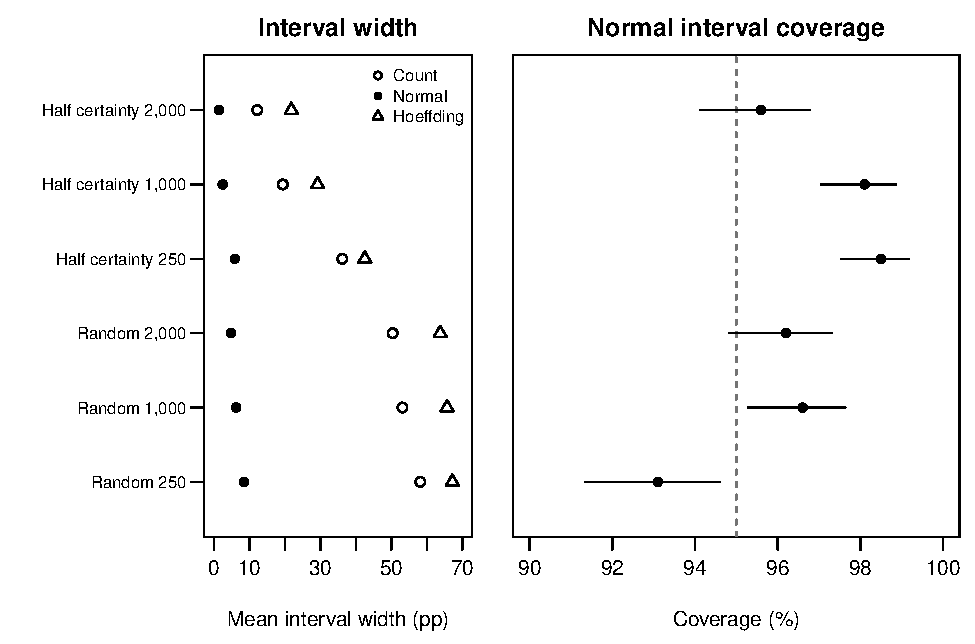
\includegraphics[width=\linewidth]{../figs/audit_comparison.pdf}
\caption{Width and coverage for the Facebook-pixel female share coefficient.
Rows compare audit budgets and designs in the fixed browsing frame. Left:
mean interval width in percentage points over 1,000 audits. Right: normal
interval coverage, with exact 95\% binomial Monte Carlo intervals and a dashed
95\% reference. Count and Hoeffding intervals covered in every simulated draw.
``Half certainty'' audits the largest absolute influences with half the budget.
Count intervals cover all contrasts of this outcome simultaneously; direct
intervals target the declared coefficient. The randomness is domain auditing;
users and predictions are held fixed.}
\label{fig:audit}
\end{figure}

Count projection covered the target in every replication but never excluded
zero. Its intervals were much wider than the approximate normal intervals; the
conservative direct Hoeffding intervals were wider still
(Figure~\ref{fig:audit}). Normal coverage in the smallest entirely
random design was \SmallAuditCoverage{}\%, with Monte Carlo interval
$[\SmallAuditCoverageLower{},\SmallAuditCoverageUpper{}]$\%, below the nominal
level. With 2,000 audited domains and half assigned to the certainty head,
normal coverage was \LargeAuditCoverage{}\% and mean width was
\LargeAuditWidth{} percentage points. These results support retaining the
locations and influences of errors, rather than treating their counts as a
sufficient validation product. They neither establish normal validity for
other outcomes nor an optimal allocation rule. Appendix~\ref{app:audit}
reports every design and method.

\subsection{Finer validation summaries}
Proposition~\ref{prop:sufficient} suggests retaining more information about
influence within a validation table. In a declared follow-up after examining
the initial audit results, we refine predicted-label strata by splitting the
ranks of signed weights into one, five, or twenty-five bins. The resulting
partitions have two, ten, or fifty strata. They use the same fixed prediction
vector and coefficient as the audit illustration. For each partition,
Table~\ref{tab:refinement} separates the identification width if every stratum's
error count were known exactly from the mean confidence-interval width when
those counts must be learned using 1,000 audited domains. The latter allocates
samples proportionally across strata, with at least two observations per
noncensus stratum, and uses 1,000 audit repetitions.

\begin{table}[htbp]
\centering\small
\caption{Refining validation reduces ambiguity but divides the audit budget}
\label{tab:refinement}
\begin{tabular}{rrrr}
\toprule
Strata & Exact-count width (pp) & Audit width (pp) & Coverage (\%) \\
\midrule
2 & 49.7 & 53.2 & 100.0 \\
10 & 34.7 & 47.1 & 100.0 \\
50 & 21.8 & 48.2 & 100.0 \\
\bottomrule
\end{tabular}

\par\smallskip
\begin{minipage}{\linewidth}\footnotesize
Facebook-pixel female share coefficient, fixed reference labels and imposed
predictions. Rank bins of signed influence cross predicted labels. Exact-count
width conditions on the population count in every stratum; audit width averages
95\% count-projection intervals over 1,000 domain samples of size 1,000, with
Bonferroni allocation across strata. Widths are percentage points. Coverage is
empirical; the exact binomial Monte Carlo intervals accompany the results.
No design certified the coefficient's sign.
\end{minipage}
\end{table}

Finer summaries reduce identification ambiguity, as the proposition predicts.
But the narrowest audit intervals among these partitions use ten strata, not
fifty. Learning more stratum counts from a fixed audit budget and protecting
their joint coverage offsets part of the gain. This comparison demonstrates
both a constructive use of the characterization and its practical constraint:
validation strata should preserve relevant weight differences without making
each count too imprecise. It does not select an optimal partition.


\section{Implications for correction and validation}
Under the common-rate model in Appendix~\ref{app:rates}, with known
$\alpha,\beta$ and
$\alpha+\beta\ne1$, equation~\eqref{eq:constantbias} gives an unbiased correction:
\begin{equation}\label{eq:correction}
 \widetilde T_i=\frac{\widehat T_i-\alpha V_i}{1-\alpha-\beta},\qquad
 \E[\widetilde T_i\mid C,y]=T_i.
\end{equation}
The correction is unstable when the denominator is close to zero and may return
values outside $[0,V_i]$. Clipping changes its expectation. Estimating error
rates introduces additional uncertainty shared across users; rates estimated
on unweighted domains need not transfer to weighted exposure. This is the
connection to classifier-based quantification \citep{vaz2019quantification},
with the additional requirement that the rates apply to each user's weights.

Using probabilities $q_j$ instead of hard labels yields $\sum_j c_{ij}q_j$.
Under a conditional-label model with information $\mathcal I$ that includes
browsing weights, $q_j=\Pr(y_j=1\mid\mathcal I)$ makes that sum
$\E[T_i\mid\mathcal I]$. Marginal calibration across domains alone does not
supply this conditional property for every user or group. This conditional-label
interpretation is distinct from the repeated-prediction interpretation used
above; an uncertainty calculation must choose and state its target.

Validation should match the research quantity. For individual totals, large
$c_{ij}$ magnify label errors. For a contrast, the relevant quantities are
$w^{\mathsf T}b$ and $w^{\mathsf T}\Sigma w$. Only under independent domain
errors does variance reduce to separate contributions $w_j^2v_j$; otherwise
validation must also address which influential errors move together. These
quantities can guide a labeling audit more directly than domain frequency alone. Verified labels for influential domains eliminate their
classification error if those labels are correct. Usage-weighted training is
another option, but its effect on exposure error requires validation; concentrated
weights do not by themselves establish that model performance will worsen.

Changing classification thresholds is a sensitivity analysis, not a set of
coverage-guaranteed bounds on true exposure. Winsorizing visits reduces the
influence of large weights but changes the exposure quantity being estimated.
The most useful validation reports errors in totals and in the intended
comparisons, together with uncertainty that preserves the common domain labels.

\clearpage
\begingroup
\small
\setlength{\bibsep}{3pt}
\urlstyle{same}
\raggedright
\bibliographystyle{plainnat}
\bibliography{references}
\endgroup

\clearpage
\appendix
\counterwithin{table}{section}
\counterwithin{figure}{section}
\counterwithin{equation}{section}
\renewcommand{\thetable}{\thesection\arabic{table}}
\renewcommand{\thefigure}{\thesection\arabic{figure}}
\renewcommand{\theequation}{\thesection\arabic{equation}}
\section*{Appendix}
\section{Bias and the denominators of error rates}\label{app:rates}
Let $\alpha_j$ be the probability of predicting one for a truly negative domain
and $\beta_j$ the probability of predicting zero for a truly positive domain,
conditional on the browsing design. Then
\begin{equation}\label{eq:bias}
 b_j=\alpha_j(1-y_j)-\beta_j y_j,\qquad
 \E[d_i\mid C,y]=\sum_j c_{ij}\{\alpha_j(1-y_j)-\beta_j y_j\}.
\end{equation}
False-positive rates condition on true negatives; false-negative rates condition
on true positives. Multiplying a false-positive rate by predicted positives
uses the wrong denominator. Such a calculation would instead require the
probability of a true negative conditional on a positive prediction, together
with assumptions that justify transferring that probability to the weighted
population. These conditional probabilities are not interchangeable.

If $\alpha_j=\alpha$ on negative domains and $\beta_j=\beta$ on positive domains,
\begin{equation}\label{eq:constantbias}
 \E[d_i\mid C,y]=\alpha(V_i-T_i)-\beta T_i
 =V_i\{\alpha-(\alpha+\beta)\pi_i\},\qquad \pi_i=T_i/V_i,
\end{equation}
where the share $\pi_i$ is defined for $V_i>0$. At a fixed true share, expected
bias scales with browsing volume unless the expression in braces is zero.
For $\alpha+\beta>0$, cancellation occurs at
$\pi_i=\alpha/(\alpha+\beta)$. Equal positive error rates cancel only when
half of visits are to truly positive domains. Thus the difference between
FPR and FNR alone does not determine bias. Nor does the number of distinct
visited domains: repeated visits matter through $c_{ij}$.

The common-rate assumption is stronger than knowing an average error rate on a
validation set of domains. Errors may depend on popularity, domain type, or
features associated with a particular group's browsing. In that case,
equation~\eqref{eq:bias}, with rates conditional on those features, is the
relevant expression. The bias in a share is $\E[d_i\mid C,y]/V_i$; dividing
by volume removes the mechanical scale factor, not misclassification bias.


\section{A connection to label sampling}
The same mapping supplies a remedy when a researcher can obtain verified
labels for a probability sample of domains. The companion \texttt{fewlab}
project develops sampling designs for reusable labels \citep{sood2026fewlab}.
Its regression decomposition is $H=AC$, with column $h_j$ giving the influence
of domain $j$ on the coefficient. For exposure shares, replace $C$ by its
row-normalized version. For the scalar contrast in equation~\eqref{eq:contrast},
the corresponding influence is $w_j$.

Freeze predictions $q_j$ before drawing a label sample. Let $R_j$ indicate
selection, with known inclusion probability $s_j>0$ for every domain. Conditional on the fixed population and predictions,
the difference estimator is
\begin{equation}\label{eq:difference}
 \widetilde\theta=\sum_j w_jq_j+
 \sum_j\frac{R_j}{s_j}w_j(y_j-q_j).
\end{equation}
Since $\E_R[R_j/s_j]=1$, its expectation over label sampling is
$\sum_jw_jy_j=\theta$, regardless of the classifier's errors. Verified labels
must measure $y_j$ correctly. Retraining the proxy on the same sampled labels
requires a separate argument; the fixed-proxy proof does not cover it.

Under independent Bernoulli domain sampling,
\begin{equation}\label{eq:designvariance}
 \Var_R(\widetilde\theta)=
 \sum_j\frac{1-s_j}{s_j}w_j^2(y_j-q_j)^2.
\end{equation}
The realized sample gives an unbiased variance estimator by replacing each
summand with $R_j(1-s_j)w_j^2(y_j-q_j)^2/s_j^2$.
Fixed-size or balanced designs require their joint-inclusion terms or a
justified approximation. An inaccurate proxy can increase variance relative
to omitting it, but does not introduce design bias under these assumptions.
This is uncertainty from randomized label acquisition, with $y$ and $q$ fixed;
it is distinct from the prediction-error process in equation~\eqref{eq:moments}.
Both calculations preserve the reuse of a domain label across people.


\section{Full audit comparison}\label{app:audit}
\begin{table}[!h]
\centering\small
\caption{All audit designs and methods for the focal coefficient}
\begin{tabular}{lr lrrr}
\toprule
Design & Budget & Interval & Coverage (\%) & Width (pp) & Sign (\%) \\
\midrule
Random & 250 & Count projection & 100.0 & 58.2 & 0.0 \\
Random & 250 & Direct normal & 93.1 & 8.4 & 39.6 \\
Random & 250 & Direct Hoeffding & 100.0 & 67.2 & 0.0 \\
Random & 1,000 & Count projection & 100.0 & 53.1 & 0.0 \\
Random & 1,000 & Direct normal & 96.6 & 6.3 & 32.9 \\
Random & 1,000 & Direct Hoeffding & 100.0 & 65.7 & 0.0 \\
Random & 2,000 & Count projection & 100.0 & 50.4 & 0.0 \\
Random & 2,000 & Direct normal & 96.2 & 4.8 & 34.4 \\
Random & 2,000 & Direct Hoeffding & 100.0 & 63.8 & 0.0 \\
Half certainty & 250 & Count projection & 100.0 & 36.2 & 0.0 \\
Half certainty & 250 & Direct normal & 98.5 & 5.9 & 40.6 \\
Half certainty & 250 & Direct Hoeffding & 100.0 & 42.5 & 0.0 \\
Half certainty & 1,000 & Count projection & 100.0 & 19.4 & 0.0 \\
Half certainty & 1,000 & Direct normal & 98.1 & 2.5 & 41.9 \\
Half certainty & 1,000 & Direct Hoeffding & 100.0 & 29.2 & 0.0 \\
Half certainty & 2,000 & Count projection & 100.0 & 12.2 & 0.0 \\
Half certainty & 2,000 & Direct normal & 95.6 & 1.4 & 65.0 \\
Half certainty & 2,000 & Direct Hoeffding & 100.0 & 21.8 & 0.0 \\
\bottomrule
\end{tabular}

\par\smallskip
\begin{minipage}{\linewidth}\footnotesize
Each row summarizes 1,000 domain audits. Coverage and sign certification are
percentages; width is the mean in percentage points. Sign certification means
that the interval excludes zero, irrespective of whether it covers the target.
All methods within a design use common draws. Exact binomial Monte Carlo
intervals, standard errors, and replicate results accompany the package.
\end{minipage}
\end{table}

\section{The original simulation of accumulating bias}
The original simulation draws 1,000 respondents, each with an independent
observation count uniformly distributed over the integers from 5 to 1,000.
Within respondents, independent bivariate normal pairs have zero means, unit
variances, and correlation $\rho=0.9$. The first component is truth and the
second a proxy. The original code adds $0.1$ times the respondent's sample
standard deviation of truth to every proxy observation. Table~\ref{tab:simulation}
retains those random draws and compares that specification with no added bias
and an exactly constant addition of $b=0.1$.

\begin{table}[htbp]
\centering
\small
\caption{Correlations with truth and signed error in respondent totals}
\label{tab:simulation}
\begin{tabular}{lrrrr}
\toprule
 & \multicolumn{3}{c}{Correlation} & Mean total \\
\cmidrule(lr){2-4}
Proxy & Observation & Mean & Total & error \\
\midrule
No added bias & 0.900 & 0.903 & 0.893 & 0.139 \\
Constant bias & 0.900 & 0.903 & 0.537 & 51.236 \\
Original SD-scaled bias & 0.900 & 0.901 & 0.538 & 51.239 \\
\bottomrule
\end{tabular}

\par\smallskip
\begin{minipage}{\linewidth}\footnotesize
Each row uses the same 1,000 respondents and random draws (seed 1234).
Error is proxy minus truth. Measurements are centered continuous variables,
so totals and errors are in arbitrary units. These are descriptive summaries
of one simulated dataset; the table does not estimate uncertainty in browsing data.
\end{minipage}
\end{table}

In the original specification, the observation-level correlation is
\OriginalObservationCorrelation{} and the total correlation is
\OriginalTotalCorrelation{}. Mean total error is \OriginalMeanError{}.
Adding an exactly constant bias leaves the correlations of observations and
respondent means unchanged. The SD-scaled addition only approximates a constant,
so that invariance is not exact for the original specification.

The constant-bias design has a simple population expression. Let $N$ be the
observation count, independent of the pairs $(Y_r,Z_r)$, and set
$S=\sum_{r=1}^{N}Y_r$, $\widehat S=\sum_{r=1}^{N}(Z_r+b)$. Because the pairs
have zero means and unit variances,
\begin{align}
 \Var(S)&=\E[N],&
 \Var(\widehat S)&=\E[N]+b^2\Var(N),&
 \Cov(S,\widehat S)&=\rho\E[N],\notag\\
 \Corr(S,\widehat S)&=\frac{\rho}{\sqrt{1+b^2\Var(N)/\E[N]}}.
 \label{eq:correlation}
\end{align}
The population correlation is \TheoreticalTotalCorrelation{}, compared with
\ConstantTotalCorrelation{} in the constant-bias simulation. With a fixed
observation count, bias shifts every total equally and does not change the
correlation. For nonzero means or a relation between counts and measurements,
equation~\eqref{eq:correlation} need not hold. Accumulating bias does not
universally reduce correlations.

This simulation isolates bias accumulation. Its normal draws can be negative,
so they are not literal visit counts or durations. It also generates observations
independently across respondents and does not simulate shared domain errors.
The covariance results above follow from the domain formulation, and are checked
separately by enumerating all prediction vectors in a small binary example.

\end{document}
